\section{Simulation Results and Discussion}
\subsection{Results} \label{results}
%When analyzing the generated data we focused especially on the average speed of agents, density and flow. We then use the individual indicators to draw a conclusion, which is mentioned in section \ref{summary}.
% From the data, we don’t see any clear changes from the base model. Neither by increasing nor decreasing the percentage of cyclists do we see any significant difference in speed, density or flow. This would imply that a change from 0\% to 20\% in cyclists doesn’t affect the car drivers to a great extent.
% We can see that while density has a few spikes see fig xy, it remains relatively stable. This would mean that the change of bicycles doesn't result in higher levels of congestion, nor does it provide any meaningful relief from traffic jams. 

% As for flow 

\subsubsection{Average Speed}\label{avg-speed}
\begin{wrapfigure}[9]{r}{0.45\textwidth}
  \centering
    \vspace{-1.15cm}
  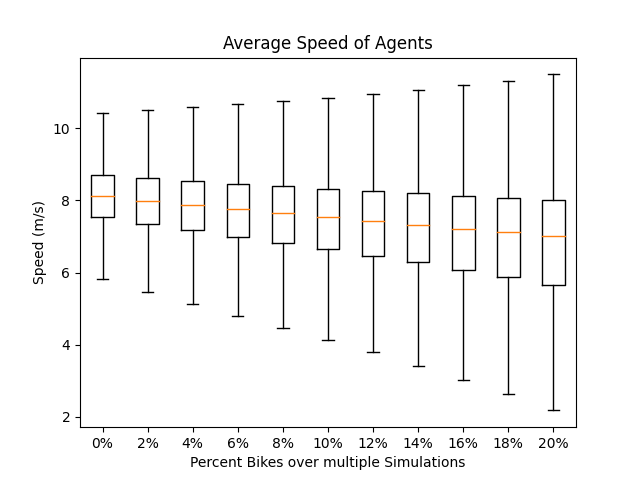
\includegraphics[width=\linewidth]{./figures/avg_speed_agent.png}
  \caption{Average Speed Agents}\label{avg-speed-agents}
\end{wrapfigure}

The graph in Fig.: \ref{avg-speed-agents} depicts the average speed of the agents for every percentage of cyclists in traffic that was simulated. There is no big change to be seen in the range of 0\% to 20\% cyclists. The average speed of all agents does however show a slightly decreasing trend. This is explainable due to the fact, that there are more cyclists on the road and these have a slower maximum velocity and are thus decreasing the average. However, due to the overtaking-mechanisms in the simulation the slower bikes also slow down the cars. This is visible when looking at the average speed of only the cars in Fig.: \ref{avg-speed-cars}. Even though there is a slight decrease in average speed, the greatest difference is from 0\% cyclists to 20\% and is not even 1$m/s$. This difference is negligible when thinking about travel time, due to the short distances, which are travelled in the city.
\vspace{-0.2cm}
\begin{figure}[H]
    \centering
    \begin{minipage}{0.45\textwidth}
        \centering
        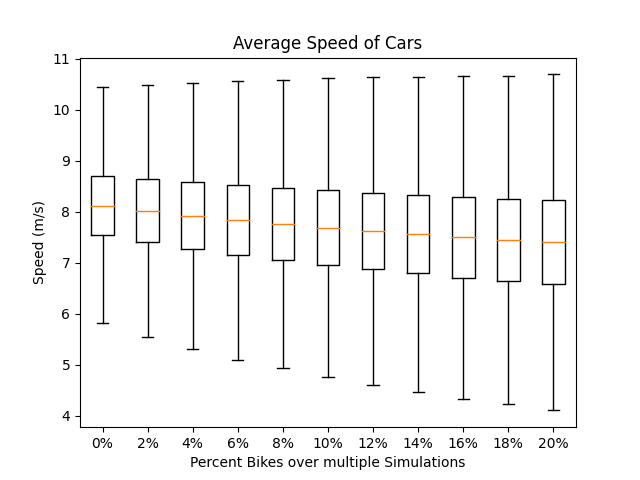
\includegraphics[width=\linewidth]{./figures/avg_speed_car.png} 
         \caption{Average Speed Cars}\label{avg-speed-cars}
    \end{minipage}
    \begin{minipage}{0.45\textwidth}
        \centering
        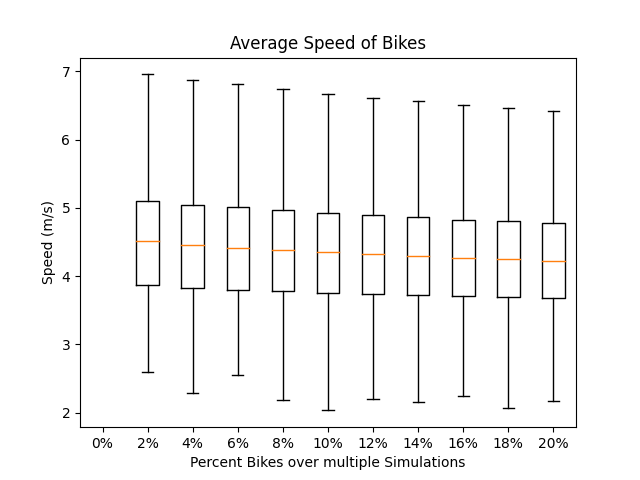
\includegraphics[width=\linewidth]{./figures/avg_speed_bike.png} 
         \caption{Average Speed Bikes}\label{avg-speed-bikes}
    \end{minipage}
\end{figure}
\vspace{-0.7cm}
\subsubsection{Density}\label{density}
The graph in Fig.: \ref{avg-density-agents} shows how the density over all agents develops with an increasing amount of cyclists. First the density slightly drops, which could be explainable by bikes being able to chose different, bike-only, routes. This allows for a wider spread of agents over the map. However then the density starts to increase a bit again. 

\begin{wrapfigure}[9]{r}{0.45\textwidth}
  \centering
    \vspace{-0.6cm}
  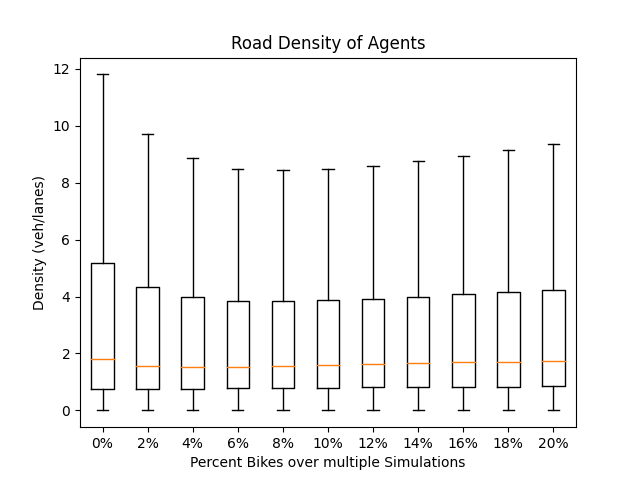
\includegraphics[width=\linewidth]{./figures/road_density_agent.png}
  \caption{Average Density of Agents}\label{avg-density-agents}
\end{wrapfigure}
This could be explained by bicycles being smaller than cars, allowing for more vehicles fitting in the same lane. If the amount of bicycles increases and they chose similar routes, the density increases for obvious reasons. This is seen in Fig.: \ref{avg-density-bikes}. The difference in average density over the different simulations would however not indicate a significant relief or worsening of congestions, since the density of cars barely changes, as seen in Fig.: \ref{avg-density-cars}.
\vspace{-0.4cm}
\begin{figure}[H]
    \centering
    \begin{minipage}{0.45\textwidth}
        \centering
        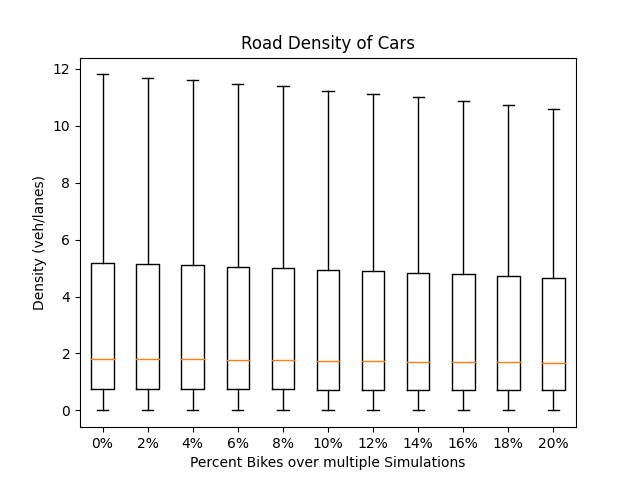
\includegraphics[width=\linewidth]{./figures/road_density_car.png} 
         \caption{Average Density of Cars}\label{avg-density-cars}
    \end{minipage}
    \begin{minipage}{0.45\textwidth}
        \centering
        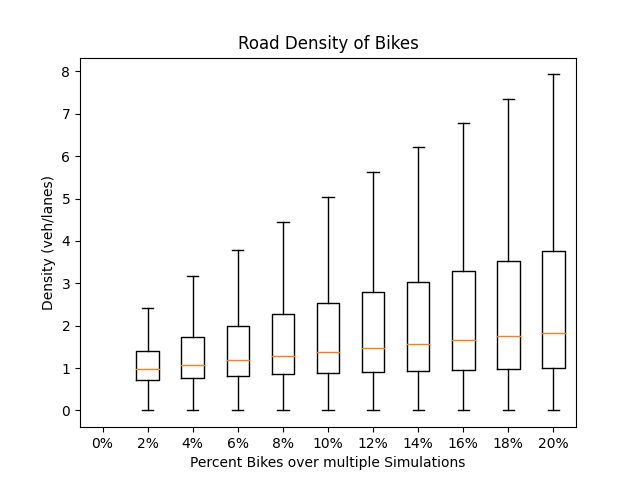
\includegraphics[width=\linewidth]{./figures/road_density_bike.png} 
         \caption{Average Density of Bikes}\label{avg-density-bikes}
    \end{minipage}
\end{figure}
\vspace{-0.6cm}
\subsubsection{Flow}\label{flow}
\begin{wrapfigure}[9]{r}{0.46\textwidth}
  \centering
    \vspace{-1.15cm}
  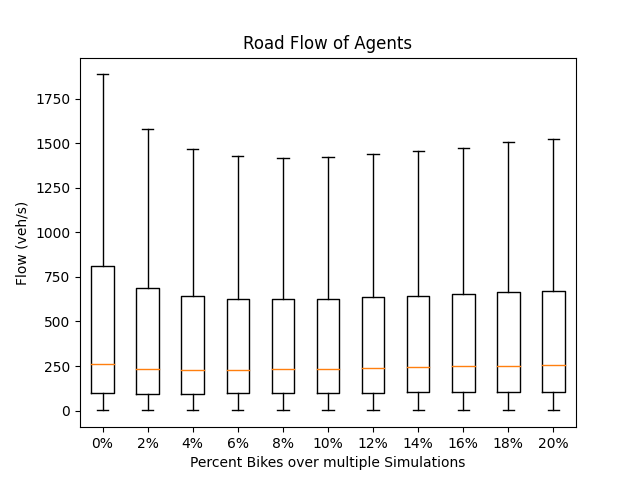
\includegraphics[width=\linewidth]{./figures/road_flow_agent.png}
  \caption{Average Flow of Agents}\label{avg-flow-agents}
\end{wrapfigure}

When looking at the average flow of agents in Fig.: \ref{avg-flow-agents} we observe a similar behavior to the density. The flow of cars decreases as seen in Fig.: \ref{avg-flow-cars} and the flow of bikes increases as seen in Fig.: \ref{avg-flow-bikes}. This makes sense, since if there are more bikes, the flow of bicycles increases. With less cars the flow of cars decreases. However, the initial drop off in flow is explicable through introducing slower bikes, needing a longer time to reach their destination and thus decreasing the flow. The following slight increase would be explainable through bicycles taking more bike-only roads, making space for cars on the normal streets, allowing for a higher flow.


\begin{figure}[H]
\vspace{-1.25cm}
    \centering
    \begin{minipage}{0.45\textwidth}
        \centering
        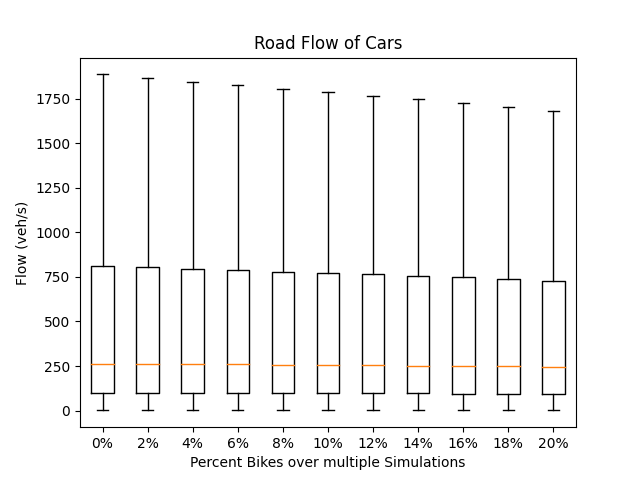
\includegraphics[width=\linewidth]{./figures/road_flow_car.png} 
         \caption{Average Flow of Cars}\label{avg-flow-cars}
    \end{minipage}
    \begin{minipage}{0.45\textwidth}
        \centering
        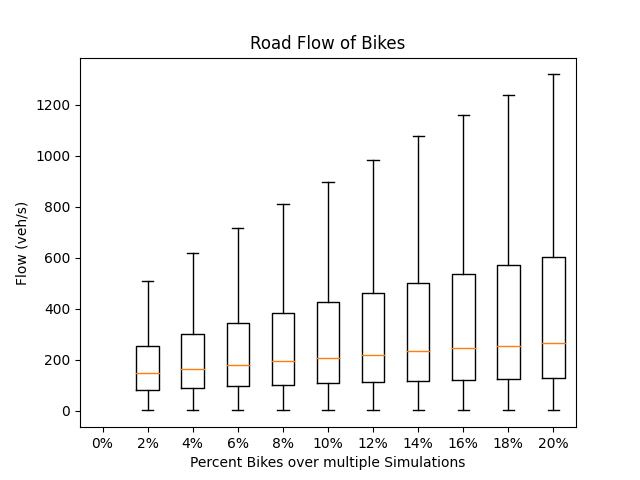
\includegraphics[width=\linewidth]{./figures/road_flow_bike.png} 
         \caption{Average Flow of Bikes}\label{avg-flow-bikes}
    \end{minipage}
\end{figure}
\vspace{-0.8cm}

\subsection{Discussion}\label{abstractions}
As with any model, assumptions and abstractions had to be made. The model is based on a map of Zurich. However, there are some limitations. One is the assumption that there are only cars and bicycles on the road, forfeiting the existence of other types of transportation, like public transport or pedestrians. This results on a lot of other factors, like street crossing pedestrians slowing down traffic, not being considered. Furthermore, events like car accidents or construction sites are not taken into consideration. Different driving styles are also not accounted for. However, due to the uniformly random values of the agent parameters, the behavior of individual agents does differ.\\
Other abstractions include the start and end points of an agent being generated completely randomly, which is not realistic. The direction of travel during a day usually forms trends due to groups of people commuting. This is not considered, since there is no data to these trends in Zurich. Furthermore, the amount of traveling people fluctuates over the course of a day. Due to the sparse data situation, this was not considered and the simulation runs on a consistent amount of agents spawned. Other behaviour of real world road users could not be accurately depicted. If there is only one lane and no separate bike lane, overtaking is not possible in our model, which is possible in some situations in real life. Also cyclists take up a whole lane in our simulation, so a cyclist can not overtake another cyclist in our simulation. This however is possible in reality. \\
The last major abstraction we made, was that all intersections are controlled by time based traffic lights. Furthermore, we assume, that when a road is incoming to an intersection, agents can use all outgoing roads of that intersection. This does not depict real world scenarios, like prohibited left turns, which occur often in Zurich.\\
Another minor simplification affects the length of the road. For the length of a  street, it is assumed, that it is a straight line between the intersections marking its end. This simplifies the calculation of its length, but extra distance as well as a reduced velocity of traffic participants in curves are not accounted for. 
